\documentclass[11pt]{article}
\usepackage{natbib}
\usepackage{array}
\usepackage{graphicx}
\usepackage{algorithm}
\usepackage{algpseudocode}
\usepackage{mathtools}
\usepackage{caption}
\usepackage{chngcntr}

\captionsetup[table]{name=Figure}
\DeclareMathOperator*{\argmax}{arg\,max}
\graphicspath{ {images/} }

\makeatletter
\renewcommand*{\thetable}{\arabic{table}}
\renewcommand*{\thefigure}{\arabic{figure}}
\let\c@table\c@figure
\makeatother 

\begin{document}
\nocite{Murphy, Wasserman, Hastie}

\title{Learning to Solve Arithmetic Word Problems Using Sentence Simplification}
\author{
	Vishal Rajpal\\
	Northeastern University\\
	rajpal.vi@husky.neu.edu\\
}
\date{}
\maketitle

\begin{abstract}
In order to respond to an arithmetic word problem correctly, one needs to understand the question to an extent that needed to determine a satisfactory answer. These are mostly semantic and are imposed by the question on its answer. Constraints from individual sentences suggest a mathematical operation and when the operators from these sentences are used collectively, the answer can be derived. To extract the constraints efficiently, a concept of Syntactic Pattern is introduced which is generated by parsing the sentence using a dependency parser. It encapsulates all the relevant information in a sentence including the subject, verb and object with its corresponding quantifiers. Another important method for this thesis which relies on syntactic patterns is Sentence Simplification. The idea is to have a subject, verb, an object and other necessary parts of speech in the sentence so that it suggests a single operation. Based on the identified patterns, a sentence may be simplified to multiple sentences. This would make the classification process easier since the sentences are less complex. To this end, it would be the classifier's job to classify the sentence to a mathematical operator. The identified operators for individual sentences are used to build a mathematical equation for the entire word problem. An empirical study is conducted on 3 datasets and we achieve results comparable with existing state-of-the-art systems.
\end{abstract}

\section{Introduction} \label{sec:introduction}
Answering arithmetic word problems has gained significant interest in recent years. The problem is attractive to natural language processing (NLP) methodologies  since the text is concise and relatively straightforward with identifiable semantic constraints. As these problems are directed towards elementary school students, they begin by describing a partial world state, followed by simple quantified updates or elaborations and end with a quantitative question. This information can be mapped to basic operations(addition, subtraction, multiplication and division) and an equation can be created that corresponds to the problem text. 

There have been a number of attempts to solve arithmetic word problems through machine learning (ML). 
All the approaches which are not template based (e.g. \citep{ARIS}, \citep{RoyTACL15} and \citep{RoyR15}) use different methods to extract similar information. Based on different ways the information is represented, an equation is generated for the problem text. The template based method of \citep{Kushman} implicitly assumes that the solution will be generated from a set of predefined equation templates. Some of these methods only solve addition and subtraction problems (e.g. \citep{ARIS} and \citep{RoyTACL15}) while others (e.g. \citep{RoyR15} and \citep{Kushman}) can solve problems for all operations.

The approach presented in this thesis can solve a general class of addition and subtraction arithmetic word problems without any predefined equation templates. In particular, it can handle an arithmetic problem as shown in Figure \ref{figure:1}.

\begin{table}[h!]
\centering
\begin{tabular}{ | m{25em} | }
\hline
\textbf{Example 1:}\\
\hline
For Halloween, Debby and her sister combined the candy they received. Debby had 32 pieces of candy while her sister had 42. If they ate 35 pieces the first night, how many pieces do they have left?\\
\hline
\end{tabular}
\caption{Example Arithmetic Word Problem.}
\label{figure:1}
\end{table}

To derive the solution to this problem, the system needs to understand that \textit{they} refers to \textit{Debby and her sister} (i.e. anaphora/pronominal resolution). Hence, the number of candies need to be summed up and then \textit{35 candies} need to be subtracted from the total number of candies. 

While a solution to these problems requires extracting information and composing numeric expressions, if the sentence is too complex it is hard to extract information accurately.

At the heart of the technical approach, the novel notion of \textit{Sentence Simplification} is involved (Section \ref{sec:sentencesimplification}). Once the sentences in the problem text are simplified, extracting information becomes easier. Each sentence in the problem is simplified to a level where it consists information which is able to be mapped to a single operator. This allows us to decompose the entire problem to a collection of simplified sentences as operator prediction problems. Each sentence represents the quantitative information with the mapped operator. These predictions (operators with the quantitative information) can be combined together to form a mathematical equation.

The approach focuses on addition and subtraction problems currently, but learning to classify operators will allow us to generalize the approach to multiplication and division problems as well. In particular, the system was able to solve Example 1 although it had never seen the problem before and required both addition and subtraction operations.

The approach is evaluated on 3 datasets, achieving competitive performance on all of them. Section \ref{sec:relatedwork} describes the related work in the area of automated arithmetic word problem solving. The theory of sentence simplification is then presented. Later the information decomposition strategy that is based on it is discussed. Section \ref{sec:logisticregressionclassifier} presents the overall computational approach, including the way classifier learns to classify simplified sentences to operators. Finally, experimental study is discussed followed with future work and conclusion.

\section{Related Work} \label{sec:relatedwork}
Most of the previous work in automated arithmetic problem solvers has focused on a restricted subset of problems.The approach described in \citep{RoyTACL15} handles problems with all basic operations but makes assumptions about the number of quantities in the problem text and the number of steps required to solve the problem. In contrast, our approach does not make any assumptions about the data in the problem text. Kushman's approach \citep{Kushman} tries to map numbers from the problem text to predefined equation templates and implicitly assume that similar equation forms have been seen in the training data. On the contrary, our system does not rely on pre-defined templates and hence is able to solve questions of type which have never been seen before.  The approach described in \citep{ARIS} might be the most related to ours. It handles addition and subtraction problems and tries to predict an operator for the verb in the problem text. Hence, it requires additional annotated data for verb categories. Our approach uses the information of the verb present in the sentence and handles addition and subtraction problems for now, but there is no requirement of additional annotated data. Refer to Section \ref{sec:features} for how the information from verbs is used as a feature. 

Most of the methods mentioned above are able to solve problems with all basic operations but our approach is easily generalizable to all the operators and also it performs competitevely compared to all other approaches. 

\section{Arithmetic Problem Representation}\label{sec:problemrepresentation}

Our approach addresses word problems that include addition and subtraction operations. Given a problem text, multiple fragments are extracted from it  where each fragment is a simplified version of the information presented in the sentence. We refer to these fragments as simplified sentences. Each fragment is represented based on the Parts of Speech it contains. The parts of speech we consider in our representation are as follows:


\textbf{Adjective:} A problem text might have multiple types of same entities. Consider the example presented in Figure \ref{figure:2}:

 \begin{table}[h!]
\centering
\begin{tabular}{ | m{25em} | }
\hline
 \textbf{A pet store had 13 siamese cats and 5 house cats.}\\
\hline
 siamese cats\\
\hline
house cats.\\
\hline
\end{tabular}
\caption{Entities with Adjective.}
\label{figure:2}
\end{table}

Though the sentence has \textit{cats} as the noun, but based on the adjectives\textit{(siamese and house)} there were \textit{siamese cats} and \textit{house cats}.
\vspace{4mm}

\textbf{Cardinal:} Cardinals are the numbers present in the problem text. We associate them to nouns based on the index at which they occur. Mostly, they occur before the noun and hence associating it is not difficult. Sometimes, the cardinal is a reference to an already occured noun. Consider Figure \ref{figure:3} for an example:

\begin{table}[h!]
\centering
\begin{tabular}{ | m{25em} | }
\hline
\textbf{He bought 2 games from a friend and bought 5 more at a garage sale.}\\
\hline
2 games\\
\hline
5 games\\
\hline
\end{tabular}
\caption{Entity with Cardinal Numbers.}
\label{figure:3}
\end{table}

\textit{5 more} in the sentence refers to games. We associate this to the last quantified noun encountered in the sentence.
\vspace{4mm}

\newpage

\textbf{Conjunction:} Conjunctions are stored mainly to simplify the sentence. Most importantly, the index at which it occurs in the sentence plays a crucial role in creating simplified sentences. Refer to Figure \ref{figure:8} for an example.
\vspace{4mm}

\textbf{Determiner:} Determiner by definition is \textit{a modifying word that determines the kind of reference a noun or a noun group has.} 

\begin{table}[h!]
\centering
\begin{tabular}{ | m{25em} | }
\hline
\textbf{There are 28 students and every student has their own lunchbox.}\\
\hline
\textit{Every} is a determiner\\
\hline
\end{tabular}
\caption{Sentence with Determiner.}
\label{figure:4}
\end{table}

In the example presented in Figure \ref{figure:4}, \textit{Every} is a determiner and when considering it, our system will be able to extract the information that there are \textit{28 lunchboxes}.
\vspace{4mm}

\textbf{Existential/Expletive:} Since, existentials indicate the existence or presence of something, they are an important part of speech for our system. Also, when the sentences are simplified, the existentials are added to the fragments which don't have them. Refer to Section \ref{sec:sentencesimplification} for more details.

\begin{table}[h!]
\centering
\begin{tabular}{ | m{25em} | }
\hline
\textbf{There are 11 rulers and 34 crayons in the drawer.}\\
\hline
There are 11 rulers in the drawer.\\
\hline
There are 34 crayons in the drawer.\\
\hline
\end{tabular}
\caption{Simplified sentences based on Existential.}
\label{figure:5}
\end{table}

In the example in Figure \ref{figure:5}, after the split based on conjunction \textit{and} the expletive \textit{There} is added to the fragment after the conjunction.
\vspace{4mm}

\textbf{Noun:} Nouns are important for answering the arithmetic word problems. Each problem text has some nouns in form of a subject \textit{(acting entity)} or an object \textit{(Entity that is acted upon by the subject)}. All the nouns are extracted from the simplified sentence and stored as a list. 
\vspace{4mm}

\textbf{Preposition:} Prepositions are helpful to keep track of location or time. Also, when simplifying sentences based on conjunctions, we add prepositions to the fragments which are missing them. Refer to the Section \ref{sec:sentencesimplification} for more details and example.
\vspace{4mm}

\newpage

\textbf{Verb:} Verbs are important for out system to predict the type of action taken by the subject. Determining the kind of action helps to predict an operation. More details on this in Section \ref{sec:features}.
\vspace{4mm}

\textbf{WHAdverb:} Existence of a WHAdverb mostly indicates the beginning of a question. Hence, having the WHAdverb in our representation helps us in the classification process. Refer to the Section \ref{sec:features}.

\section{Sentence Simplification and Problem Decomposition} \label{sec:sentencesimplification}
Sentences in an arithmetic word problem are sometimes complex. Hence, it is difficult to extract information from such sentences. Even more challenging is to predict the impact of the sentence on the result. 

\begin{table}[h!]
\centering
\begin{tabular}{ | m{25em} | }
\hline
\textbf{Example 2:}\\
\hline
\begin{math}s\end{math}: Henry had 11 dollars. For his birthday he got 18 more dollars but spent 10 on a new game. How much money does he have now?\\
\hline
\begin{math}s_{1}\end{math}: Henry had 11 dollars.\\
\hline
\begin{math}s_{2}\end{math}: For his birthday he got 18 more dollars but spent 10 on a new game.\\
\hline
\begin{math}s_{3}\end{math}: How much money does he have now?\\
\hline
\end{tabular}
\caption{Example Arithmetic Word Problem.}
\label{figure:6}
\end{table}

Consider the example presented in Figure \ref{figure:6}. Sentence \begin{math}s_{2}\end{math} is complex for a machine learning algorithm. It has addition and subtraction operation in a single sentence. Our idea is to simplify the sentence to multiple simple sentences so that each simplified sentence has a single operation. The simplified sentences for \begin{math}s_{2}\end{math} are listed in Figure \ref{figure:7}.

\begin{table}[h!]
\centering
\begin{tabular}{ | m{25em} | }
\hline
 \textbf{For his birthday he got 18 more dollars but spent 10 on a new game.}\\
\hline
 For his birthday he got 18 more dollars.\\
\hline
He spent 10 dollars on a new game.\\
\hline
\end{tabular}
\caption{Simplified Sentences.}
\label{figure:7}
\end{table}

We create a mapping for each sentence in the problem text to its simplified sentences by extracting their relational dependencies from the Stanford dependency parser\footnote{http://stanfordnlp.github.io/CoreNLP/ }. Currenly, our system simplifies sentences based on conjunctions. There are certain rules when simplifying the sentence.

\subsection{Rules for simplifying sentences based on conjunctions.}\label{sec:simplifyingrules}
 When a conjunction is encountered, our system attempts to create two simplified sentences from the actual sentence. The first sentence is the part before the conjunction while the second sentence is the part after the conjunction.

Notably, after the split there may be some words which would be required in the second sentence. Consider the example in Figure \ref{figure:8}.

\begin{table}[h!]
\centering
\begin{tabular}{ | m{25em} | }
\hline
The school cafeteria ordered 42 red apples and 7 green apples for students lunches.\\
\hline
\end{tabular}
\caption{Example Sentence}
\label{figure:8}
\end{table}

Given a sentence \begin{math}s\end{math} from problem text \begin{math}p\end{math}, after simplification process it will have  \begin{math}n\end{math} simplified sentences i.e. \begin{math}<s_{1},..., s_{n}>\end{math}. In the sentence \begin{math}s\end{math}, the split based on conjunction \textit{and} will result in two sentences. 

\begin{math}s_{1}\end{math}:\textit{The school cafeteria ordered 42 red apples}

\begin{math}s_{2}\end{math}:\textit{7 green apples for students lunches}


\begin{math}s_{1}\end{math} will have a subject while \begin{math}s_{2}\end{math} will not have a subject and a verb making it an improper sentence. Hence, there are some rules for adding words to simplified sentences:

\subsubsection{Rules for adding words to simplified sentences.}\label{sec:secondsentencesimplification}
\begin{enumerate}
\item \label{rule:1}
If \begin{math}s_{1}\end{math} starts with an existential and has a verb after it and if \begin{math}s_{2}\end{math} does not have either expletive or verb, distribute them to \begin{math}s_{2}\end{math}. Consider the example in Figure \ref{figure:9}:

\newpage
\begin{table}[h!]
\centering
\begin{tabular}{ | m{25em} | }
\hline
 \textbf{\begin{math}s\end{math}: There were 2 siamese cats and 4 house cats.}\\
\hline
\begin{math}s_{1}\end{math}: There were 2 siamese cats.\\
\hline
\begin{math}s_{2}\end{math}: There were 2 house cats.\\
\hline
\end{tabular}
\caption{Example sentence for Rule \ref{rule:1}}.
\label{figure:9}
\end{table}

The expletive and verb were added to \begin{math}s_{2}\end{math} based on the simplification rule mentioned above.

\item \label{rule:2}
If \begin{math}s_{1}\end{math} starts with a noun, and if \begin{math}s_{2}\end{math} starts with a verb, the noun from the former will be distributed to the latter. Refer to an example in Figure \ref{figure:10}.

\begin{table}[h!]
\centering
\begin{tabular}{ | m{25em} | }
\hline
 \textbf{\begin{math}s\end{math}: Joan ate 2 oranges and threw 3 apples.}\\
\hline
\begin{math}s_{1}\end{math}: Joan ate 2 oranges.\\
\hline
\begin{math}s_{2}\end{math}: Joan threw 3 apples.\\
\hline
\end{tabular}
\caption{Example sentence for Rule \ref{rule:2}.}
\label{figure:10}
\end{table}

\item  \label{rule:3}
If \begin{math}s_{1}\end{math} starts with a noun and \begin{math}s_{2}\end{math} has a \textit{noun verb} pattern, do nothing.

\begin{table}[h!]
\centering
\begin{tabular}{ | m{25em} | }
\hline
 \textbf{\begin{math}s\end{math}: Tom has 9 yellow balloons and Sara has 8 yellow balloons.}\\
\hline
\begin{math}s_{1}\end{math}: Tom has 9 yellow balloons.\\
\hline
\begin{math}s_{2}\end{math}: Sara has 8 yellow balloons.\\
\hline
\end{tabular}
\caption{Example sentence Rule  \ref{rule:3}.}
\label{figure:11}
\end{table}

In the example presented in Figure \ref{figure:11}, No words from \begin{math}s_{1}\end{math} were added to \begin{math}s_{2}\end{math} since it had the \textit{noun verb (Sara has)} pattern.

\item \label{rule:4}
If \begin{math}s_{2}\end{math} contains a preposition at the end and \begin{math}s_{1}\end{math} does not, it will be distributed from \begin{math}s_{2}\end{math} to \begin{math}s_{1}\end{math}. Consider the example presented in Figure \ref{figure:12}:

\newpage
\begin{table}[h!]
\centering
\begin{tabular}{ | m{25em} | }
\hline
 \textbf{\begin{math}s\end{math}: Joan found 6 seashells and Jessica found 8 seashells on the beach.}\\
\hline
\begin{math}s_{1}\end{math}: Joan found 6 seashells on the beach.\\
\hline
\begin{math}s_{2}\end{math}: Jessica found 8 seashells on the beach.\\
\hline
\end{tabular}
\caption{Example sentence for Rule  \ref{rule:4}.}
\label{figure:12}
\end{table}

After splitting the sentence based on \textit{and}, the preposition and the words after it \textit{on the beach} were added to the first sentence.

\item
Based on the output by the dependency parser and our rules, there might be some words which might not have been identified. But we still need those words in the simplified sentences. Therefore, the sentence simplification system identifies all such words. If these words appear before the conjunction, they are added to \begin{math}s_{1}\end{math} at the correct index and if they appear after the conjunction, they are added to \begin{math}s_{2}\end{math}.

\end{enumerate}


\subsection{Syntactic Pattern}\label{sec:syntacticpattern}
In this thesis, a concept known as Syntactic Pattern is introduced which is basically a summarized information about a fragment. It is a pattern consisting of the initials of the parts of speech which appear in the fragment. The initials are arranged in the order in which the words appear in the sentence. Consider the picture in Figure \ref{figure:13}:

\begin{figure}[h!]
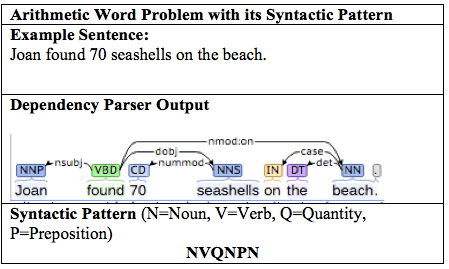
\includegraphics[width=0.8\textwidth]{Figure1}
\centering
\caption{Example sentence of a word problem and its syntactic pattern.}
\label{figure:13}
\end{figure}

As in Figure \ref{figure:13}, the pattern \textit{NVQNPN} consists of the initials of the parts of speech in the sentence in their appearance order. This pattern is helpful in many ways:

\textbf{Grouping Multiple Fragments:} Many fragments will have a similar syntactic pattern. Our findings suggest that the fragments having a similar pattern perform similar type of operation. Refer to the example in Figure \ref{figure:14}:

\begin{table}[h!]
\centering
\begin{tabular}{ | m{16em} | m{6em} | m{6em} |}
\hline
\textbf{Example Sentence} & \textbf{Syntactic Pattern} & \textbf{Operation}\\
\hline
Joan found 70 seashells on the beach. & \textbf{NVQNPDN} & Addition \\
\hline
Mary took 10 rulers from the drawer. & \textbf{NVQNPDN} & Subtraction\\
\hline
Dave gave some rulers to Mary. & \textbf{NVDNPN} & Assignment\\
\hline
\end{tabular}
\caption{Example sentences and their Syntactic Pattern.}
\label{figure:14}
\end{table}
 
The first two examples have the same pattern and hence perform a similar operation \textit{Addition and Subtraction}. The last sentence has a different pattern and performs an assignment operation which is different than the basic math operations. Refer to Section \ref{sec:features} for more information.

\textbf{Metadata:} The pattern acts as a metadata for our fragments. Based on our representation, it is easy to determine if the fragment consists of any conjunction, quantities or any other parts of speech. 
\begin{table}[h!]
\centering
\begin{tabular}{ | m{20em} | m{6em} |}
\hline
\textbf{Example Sentence} & \textbf{Syntactic Pattern}\\
\hline
Joan found 70 seashells on the beach. &  \textbf{NVQNPDN} \\
\hline
 & \\
\hline
\textbf{Parts of Speech} & \textbf{Count}\\
\hline
Adjective & 0 \\
\hline
Cardinal (Quantity) & 1\\
\hline
Conjunction & 0\\
\hline
Determiner & 1\\
\hline
Existential/Expletive & 0\\
\hline
Noun & 3\\
\hline
Preposition & 1\\
\hline
Verb & 1\\
\hline
WHAdverb & 0\\
\hline
\end{tabular}
\caption{Decomposing the Syntactic Pattern.}
\label{metadata}
\end{table}

 To be able to extract this information in a simple way is helpful to our system. Refer to Section \ref{sec:features} for more details.

\section {Operator Prediction Classifier}\label{sec:predictionclassifier}
We train 4 Logistic Regression binary classifiers each for different operators \textit{(+, -, =, ?)}. We then use one versus all technique to combine the results from the binary classifiers. Given a fragment \textit{f} from a problem text \textit{p}, we determine which one of the operations, fragment \textit{f} is most likely to perform. We have around 94 questions from which 301 fragments were extracted. We label these fragments and perform a 5-fold cross validation to train our classifier. Refer to Figure \ref{fig:trainingdatadistribution} for distribution of fragments among class labels.

\begin{table}[h!]
\centering
\begin{tabular}{ | m{6em} | m{6em} |}
\hline
\textbf{Class Label} & \textbf{Count}\\
\hline
+ & 137\\
\hline
- & 57\\
\hline
= & 13\\
\hline
? & 94\\
\hline
Total & 301\\
\hline
\end{tabular}
\caption{Count of traning fragments for each class label.}
\label{fig:trainingdatadistribution}
\end{table}

\subsection {Features}\label{sec:features}

\subsubsection{Syntactic Patterns}\label{sec:featuressyntacticpattern}
From 301 training fragments, we were able to extract 125 syntactic patterns. This proves that multiple fragments had same patterns. We use these patterns as individual features. For a given fragment, the pattern to which it belongs is set\textit{(on)} and the other patterns are not set\textit{(off)}. We use one-hot encoding approach for pattern features.

\subsubsection{Occurence Features}\label{sec:featuresoccurence}

\textbf{Relation based occurence features:} Dependency relations in a fragment depict its structure. Presence of some dependency relations is useful for the classifier to predict operations. Particularly, \textit{nmod:poss} relation if exists in the fragment, can determine information about a subject possessing an object. \textit{nmod:of} helps to differentiate between two nouns of same kind. The examples are listed in Figure \ref{figure:15}:

\begin{table}[h!]
\centering
\begin{tabular}{ | m{25em} | }
\hline
 \textbf{Sam had 20 pieces of cake and 10 pieces of butter in his plate.}\\
\hline
\textit{nmod:of(pieces-4, cake-6)}\\
\hline
\textit{nmod:of(pieces-9, butter-11)}\\
\hline
\textit{nmod:poss(plate-14, his-13)}\\
\hline
\end{tabular}
\caption{Example relations in the fragment.}
\label{figure:15}
\end{table}

It is easy to see that presence of these relations is mostly in the fragments in which some operation takes place.

\textbf{Pattern based occurence features:} Occurence of some specific sub pattern in the syntactic pattern of the fragment can be helpful. Specifically, \textbf{NVQN} and \textbf{QN} are used as features for the classifier. Their presence again indicates some operation. Consider the example in Figure \ref{figure:16}:

\begin{table}[h!]
\centering
\begin{tabular}{ | m{20em} | m{5em} |}
\hline
 \textbf{Sentence} & \textbf{Syntactic Pattern}\\
\hline
\begin{math}s_{1}\end{math}: George received 30 dollars. & \textbf{NVQN} \\
\hline
\begin{math}s_{2}\end{math}: 18 cupcakes were sold. & \textbf{QNVV} \\
\hline
\end{tabular}
\caption{Example occurence of a sub pattern.}
\label{figure:16}
\end{table}

In \begin{math}s_{1}\end{math}, both \textit{NVQN} and \textit{QN} appear. While, in \begin{math}s_{2}\end{math} \textit{QN} appears. Presence of quantity in a fragment is more likely to suggest an operation. 

\textbf{Word based occurence features:} Occurence of some particular words in the fragment help the classifier. Figure \ref{figure:17} has the list of some words and description of how they are helpful:

\begin{table}[h!]
\centering
\begin{tabular}{ | m{5em} | m{15em} | m{15em} | }
\hline
 \textbf{Word} & \textbf{Description} & \textbf{Example}\\
\hline
\textit{now} & Suggests a resulting output after some operations. & Fruits were distributed to 28 students. There are now 12 fruits remaining. \\
\hline
\textit{most, several, some} & Suggest an unknown quantity in the fragment. & Joan gave some of her seashells to Sam. \\
\hline
\end{tabular}
\caption{Examples for occurence of specific words.}
\label{figure:17}
\end{table}

\subsubsection{Count based Features}\label{sec:featurescountbased}
Based on our analysis we found that having a count of some parts of speech occuring the the syntactic pattern proves to be helpful to the classifier in learning accurately. Refer to Figure \ref{figure:18} for more details:

\begin{table}[h!]
\centering
\begin{tabular}{ | m{5em} | m{25em} |}
\hline
\textbf{Feature} & \textbf{Description} \\
\hline
 Number of Nouns. & Generally a fragment having 2 nouns \textit{subject and object} is more likely to be predicted to addition or subtraction operation.\\
\hline
Number of Prepositions. & A single preposition(such as \textit{from} or \textit{to} is suggesting the movement of object.\\
\hline
Number of Verbs. & If there are no verbs in the fragment, there should ideally be no actions performed.\\
\hline
Number of Quantities. & If there is no quantity in the fragment, it is more likely that math operations have not been performed.\\
\hline
\end{tabular}
\caption{Count based Features.}
\label{figure:18}
\end{table}

\subsubsection{Verb similarity based features}\label{sec:featuressimilaritybased}
Verbs are important to determine the kind of action the fragment is trying to perform. The verbs present in the sentence are given as an input to WordNet\textit{(a large lexical database of English. Nouns, verbs, adjectives and adverbs are grouped into sets of cognitive synonyms)} \citep{WordNet} and Word2Vec(\textit{Computes high-quality word vector representations of words from huge datasets with billions of words}) \citep{Word2Vec}. 

For an input verb \textit{v}, WordNet outputs a set of categories \textit{($c_{1}$, $c_{2}$,...,$c_{n}$)} to which the verb is most likely to belong. We shortlisted 8 verb categories as listed in Figure \ref{figure:19} which can prove helpful to our system:

\newpage
\begin{table}[h!]
\centering
\begin{tabular}{ | m{15em} | }
\hline
 \textbf{Verb Categories.}\\
\hline
verb.possession\\
\hline
verb.change\\
\hline
verb.communication\\
\hline
verb.consumption\\
\hline
verb.contact\\
\hline
verb.creation\\
\hline
verb.motion\\
\hline
verb.weather\\
\hline
\end{tabular}
\caption{Shortlisted Verb Categories.}
\label{figure:19}
\end{table}

We use Word2Vec to get 3 nearest words to the verb and send those words as an input to WordNet to get the verb categories they belong. We normalize the results for these 3 words and the results for the verb itself. Hence, In total we have 8 normalized similarity based features(verb categories).

\textbf{Step 1:} Pass the identitified verb in the sentence as an input to WordNet. Refer to Figure \ref{wordnetexample} for an example:

\begin{table}[h!]
\centering
\begin{tabular}{ | m{30em} |}
\hline
\textbf{Example Sentence:} Joan baked 10 cupcakes.\\
\hline
 \textbf{Verb:} baked\\
\hline
\textit{Sense 1 \textless verb.change\textgreater bake =\textgreater \textless verb.change\textgreater cook}\\
\hline
\textit{Sense 2 \textless verb.creation\textgreater bake =\textgreater \textless verb.creation\textgreater create from raw material, create from raw stuff}\\
\hline
\textit{Sense 3 \textless verb.change\textgreater broil1, bake2 =\textgreater \textless verb.change\textgreater heat1, heat up}\\
\hline
\end{tabular}
\caption{Using WordNet on the Verb.}
\label{wordnetexample}
\end{table}

\textbf{Step 2:} Get the top 3 closest words to the verb using Word2Vec. Figure \ref{word2vecexample} consists an example:

\begin{table}[h!]
\centering
\begin{tabular}{ | m{30em} |}
\hline
Word2Vec for verb: \textit{baked} \\
\hline
["unbaked", 0.602738618850708]\\
\hline
["cooked", 0.6022148728370667]\\
\hline
["bakes", 0.5771548748016357]\\
\hline
\end{tabular}
\caption{Using WordNet on the Verb.}
\label{word2vecexample}
\end{table}

\textbf{Step 3:} Pass the closest words as an input to WordNet to identify their verb categories. Similar to Figure \ref{wordnetexample}, each word will have their own distribution of categories. Hence, we normalize results between 8 categories as in Figure \ref{normalized}.

\begin{table}[h!]
\centering
\begin{tabular}{ | m{20em} | m{5em} |}
\hline
\textbf{Verb Category} & \textbf{Probability} \\
\hline
verb.possession & 0\\
\hline
verb.change & 0.6\\
\hline
verb.communication & 0\\
\hline
verb.consumption & 0\\
\hline
verb.contact & 0\\
\hline
verb.creation & 0.4\\
\hline
verb.motion & 0\\
\hline
verb.weather & 0\\
\hline
\end{tabular}
\caption{Normalized results for verb categories.}
\label{normalized}
\end{table}

Alongside other features, these values are also used as features for our classifier.

\subsection{Logistic Regression Classifier}\label{sec:logisticregressionclassifier}

Logistic Regression (LR) tries to fit a model of the form \begin{math} p(y|X) \end{math} which directly models the mapping from input \begin{math}X\end{math} to output \begin{math}y\end{math}. Since, it discriminates between class labels it is known as a discriminative classifier. LR corresponds to following binary classification model \citep{Murphy}:

\begin{equation} p(y|X,W) = Ber(y|sigm(W^{T}X)) \end{equation}

Each fragment will to be classified to one of the operators/class mentioned in Figure \ref{figure:20}:

\begin{table}[h!]
\centering
\begin{tabular}{ | m{5em} | m{20em} |}
\hline
 \textbf{Operator} & \textbf{Description}\\
\hline
+ & Addition operation. \\
\hline
- & Subtraction operation. \\
\hline
= & Assignment operation. \\
\hline
? & The fragment is asking some question.\\
\hline
\end{tabular}
\caption{Logistic Regression output classes.}
\label{figure:20}
\end{table}

Each class has its own binary LR classifier. We use an algorithm known as \textbf{Stochastic Gradient Descent (SGD)} to train all the four LR classifiers. Refer to the algorithm presented in \ref{figure:21}:

\begin{algorithm}
\caption{Stochastic Gradient Descent (SGD)}
\label{figure:21}
\textit{Initialize $\theta$, $\eta$, b;}
\begin{algorithmic}
\Repeat 
\State Randomly permute data;
\For{\texttt{i = 1:N}}
\State s = sigm($X_{i}$);
\State updateWeightVector(s, $X_{i}$);
\State g = updateGradient(s, $y_{i}$);
\State Update b;
\EndFor
\Until
\end{algorithmic}
\end{algorithm}

We have 3 parameters as shown above: $\theta$(weight vector), $\eta$(learning rate) and b(bias). In SGD, we repeatedly run through the training set, and each time we encounter a training example, we update the parameters according to the gradient of the error with respect to that single example only. We calculate the error based on sigmoid function value. A sigmoid function is a mathematical function having an \textit{S} shaped curve \textbf{sigmoid curve}. Figure \ref{figure:21} shows the sigmoid function.

\begin{figure}[h!]
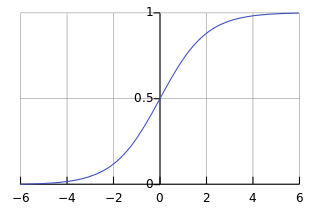
\includegraphics[width=0.7\textwidth]{Figure2}
\centering
\caption{Sigmoid Curve.}
\label{figure:21}
\end{figure}

The function is defined by the below formula:
\begin{flalign*}
&S(t) = \frac{1}{1 + e^{-t}} \\
&t = \theta_{T}X \\
&\theta \rightarrow \textit{Weight vector} \\
&X \rightarrow \textit{Feature vector for an example}
\end{flalign*}

The function has finite limits and approaches negative infinity from the left side and to infinity from the right.  When the algorithm encounters an example, it updates the weight for a particular feature in the weight vector if the feature is set in the current example's feature vector. Based on the sigmoid function value, the gradient and all the parameters are updated. 

\subsubsection{Training the classifier}\label{sec:classifiertraining}
We train our four LR binary classifiers on 301 operator labeled fragments and then use one versus all\textit{(OvA)} technique to combine the results from all four of them. The OvA strategy involves training a single classifier per class\textit(4 operators in our case). The samples of that class are treated as positive and all other samples are treated as negative. For example, when training a classifier for \textbf{+} operator, the training samples having \textbf{+} label are positive and samples having other labels i.e. \textbf{-, =, ?} are considered negative. This strategy requires the base classifiers to produce a real-valued confidence score for its decision, rather than just a label. Once we have a real valued score from all the base classifiers, the technique predicts a single class using the below mechanism:

\begin{equation}
y^{\prime} = \argmax_{k = 1,...,K} f_{k}(x)
\end{equation}

\subsubsection{Precision and Recall}\label{sec:precisionandrecall}
Our testing data consists of 55 fragments. Figure \ref{figure:22} consists of the distribution of fragments among all the operations and their precision and recall values:


\begin{table}[h]
\begin{center}
\begin{tabular}{|c|c|c|c|}
\hline
\bf Operation & \bf No. of instances & \bf Precision & \bf Recall \\
\hline
+ & 32 & 95.83\% & 71.87\% \\
\hline
- & 9 & 40\% & 66.66\% \\
\hline
= & 2 & 50\% & 50\% \\
\hline
? & 15 & 82.35\% & 93.33\% \\
\hline
\end{tabular}
\end{center}
\label{figure:22}
\caption{Precision and Recall}
\end{table}

The higher precision and recall of operation \textbf{?} is well understood as there were features such as the presence of an WHAdverb which made it easy for the classifier to predict them accurately. Whereas, for \textbf{+} the verb based similarity features played an important role. For operations \textbf{-} and \textbf{=} its not really correct to judge since there were less number of testing fragments.

\subsection{Experimental Results}\label{sec:experimentalresults}
In this section, we evaluate the proposed method on publicly available datasets of arithmetic word problems. We show the parameter setup of our LR classifiers. Lastly, we evaluate the performance of the full system.

\subsubsection{Datasets}\label{sec:datasets}
We evaluate our system on three datasets, each of which comprise a different category of arithmetic word problems.

\begin{enumerate}
\item \textbf{A12 Dataset:} This dataset is a collection of 395 addition and subtraction problems, released by \citep{ARIS}. They perform a 3-fold cross validation, with every fold containing problems from different sources. This helps to evaluate robustness to domain diversity. To evaluate our system, we follow the same evaluation setting.

\item \textbf{IL Dataset:} This is a collection of arithmetic problems released by \citep{RoyTACL15}. Each of these problems can be solved by performaing one operation. This dataset consists of problems having all basic operations but we only consider addition and subtraction problems. Though, we cannot compare our results to them, we still achieve a competitive accuracy on addition and subtraction problems. We use a 5-fold cross validation to evaluate on this dataset.

\item \textbf{Commoncore Dataset:} This dataset is released by \citep{RoyR15} and consists of 600 word problems. These problems similar to the IL dataset have all basic operations, but we only consider addition and subtraction problems. 200 problems have addition and subtraction operations in them. We perform 6-fold cross validation to evaluate on these problems.
\end{enumerate}


\subsubsection{Experimental Setup}\label{sec:experimentalsetup}
As explained in the Section \ref{sec:logisticregressionclassifier}, the algorithm needs 2 parameters \begin{math}\eta\end{math} and \begin{math}b\end{math}. Tthe values we use for all the four classifiers are mentioned in Figure \ref{figure:23}:

\begin{table}[h]
\begin{center}
\begin{tabular}{|c|c|c|}
\hline
\textbf{Operator} & \begin{math}\eta\end{math} & \begin{math}b\end{math} \\
\hline
+ & 0.0001 & -1.5 \\
\hline
- & 0.0005 & -1.0\\
\hline
= & 0.01 & 0.0\\
\hline
? & 0.001 & 0.0\\
\hline
\end{tabular}
\end{center}
\label{figure:23}
\caption{Parameter Values}
\end{table}

These values were decided based on performance on trial of certain values. Section \ref{sec:results} describes the results achieved on the datasets.

\subsubsection{Results}\label{sec:results}

The results in Figure \ref{figure:24} are achieved in evaluating our system on datasets mentioned above. 

\begin{table}[h!]
\begin{center}
\begin{tabular}{|c|c|c|c|}
\hline
\textbf{Approach/Datasets} & \textbf{A12} & $\textbf{IL}^{*}$ & $\textbf{CC}^{*}$ \\
\hline
 & 60\% & 72.88\% & 50\% \\
\hline
~\citep{RoyR15} & 78\% & 73.9\% & 45.2\% \\
\hline
~\citep{Kushman} & 64\% & 73.7\% & 2.3\% \\
\hline
~\citep{ARIS} & 77.7\% & - & - \\
\hline
~\citep{RoyTACL15} & - & 52.7 & - \\
\hline
\end{tabular}
\end{center}
\caption{Accuracy in correctly solving arithmetic problems.}
\label{figure:24}
\end{table}

\textit{$^{*}$These datasets contain problems for all operations. From these datasets, we have evaluated our system for addition and subctraction problems only. Hence, the results for these datasets are for informational purposes.}\\

The first row of the above table are the results achieved by our system. We achieve competitive results compared to other approaches. For IL and CC datasets we only evvaluate on addition and subtraction problems and hence the results if not be the correct comparison.

\section{Discussion}\label{sec:discussion}

Our system is generalized as it gives importance to every fragment initially and then based on its structure ignores irrelevant information. Not only verbs\citep{ARIS}, but other parts of speech play an equal role in solving arithmetic word problems. 

\subsection{Future Work}\label{sec:futurework}
\subsubsection{Multiplication and Division Problems}\label{sec:futureworkmanddproblems}
We aim to solve multiplication and division problems using a similar approach. Based on our analysis, we believe that by adding additional features and training data, multiplication and division problems could be solved.

\subsubsection{Additional Complex Parsing Rules}\label{sec:futureworkparsingrules}
Currently, our system employs some complex but mostly simpl rules to solve arithmetic problems. We aim to add more complex parsing rules to extract quantified nouns and their relations with verbs. This would help the classifier to predict operations more accurately. 

\subsubsection{Improving the Classifier}\label{sec:classifierimprovement}
We also plan to focus on improving the classifier by using some advanced machine learning methods. At this point, we have a LR classifier which performs reassonably well. This is an area to predict the operator for a fragment more accurately. We plan to consider ensembling methods in future.

\subsection{Error Analysis}\label{sec:erroranalysis}
\begin{table}[h!]
\begin{center}
\begin{tabular}{|>{\centering\arraybackslash}m{8em}|>{\centering\arraybackslash}m{20em}|}
\hline
\bf Error Type & \bf Example \\
\hline
Classification Errors (75\%) & He now has 56 books in his library. \textbf{Classified to "+" but should be "="}. \\
\hline
Parsing Issues (15\%) & Sara has 31 \textbf{red} and 15 green balloons. \\
\hline
Coreference Resolution (10\%) & When they cleaned them , they discovered that \textbf{29} were cracked. \\
\hline
\end{tabular}
\caption{Examples of different error categories and relative frequencies.}
\label{figure:25}
\end{center}
\end{table}

As per Figure \ref{figure:25}, we can see the need to improve the classifier based on the number of classification errors. There is a possibility of improvement in parsing issues by adding more rules. 

\section{Conclusion}\label{sec:conclusion}
This thesis presents a method for understanding and solving addition and subtraction arithmetic word problems. We develop a novel theoritical framework, centered around the notion of syntactic patterns and implement it to produce simplified sentences. This theory naturally leads to a solution to uniquely solve word problems - \textit{determine the quantified nouns and operation in the problem text}. The theory underlies our algorithmic solution. We show this by developing a classifier that yields strong performance on several benchmark collections. Our approach also performs equally well on multistep problems, even when it has never observed the particular problem type before.


\paragraph{Acknowledgements} \hspace{0pt} \\
I thank Kevin Small and other reviewers for guidance, motivation, helpful reviews and feedback on the work.

\newpage
\section{Appendix}

\begin{table}[h!]
\centering
\begin{tabular}{ | m{35em} | }
\hline
\begin{math}s\end{math}: \textbf{Lana picked 36 tulips and 37 roses to make flower bouquets.} \\
\hline
\begin{math}s_{1}\end{math}: Lana picked 36 tulips to make flower bouquets. \\
\hline
\begin{math}s_{2}\end{math}: Lana picked 37 roses to make flower bouquets. \\
\hline
\\
\hline
\begin{math}s\end{math}: \textbf{Carol and her mom were picking carrots from their garden.} \\
\hline
\begin{math}s_{1}\end{math}: Carol were picking carrots from their garden. \\
\hline
\begin{math}s_{2}\end{math}: Her mom were picking carrots from their garden. \\
\hline
\\
\hline
\begin{math}s\end{math}: \textbf{Megan took 15 pictures at the zoo and 18 at the museum.} \\
\hline
\begin{math}s_{1}\end{math}: Megan took 15 pictures at the zoo. \\
\hline
\begin{math}s_{2}\end{math}: Megan took 18 pictures at the museum. \\
\hline
\\
\hline
\begin{math}s\end{math}: \textbf{Ned had to wash 9 short sleeve shirts and 21 long sleeve shirts before school.} \\
\hline
\begin{math}s_{1}\end{math}: Ned had to wash 9 short sleeve shirts before school. \\
\hline
\begin{math}s_{2}\end{math}: Ned had to wash 21 long sleeve shirts before school. \\
\hline
\\
\hline
\begin{math}s\end{math}: \textbf{Faye had 46 math problems and 9 science problems for homework.} \\
\hline
\begin{math}s_{1}\end{math}: Faye had 46 math problems for homework. \\
\hline
\begin{math}s_{2}\end{math}: Faye had 9 science problems for homework. \\
\hline
\\
\hline
\begin{math}s\end{math}: \textbf{Amy had 4 music files and 21 video files on her flash drive.} \\
\hline
\begin{math}s_{1}\end{math}: Amy had 4 music files on her flash drive. \\
\hline
\begin{math}s_{2}\end{math}: Amy had 21 video files on her flash drive. \\
\hline
\\
\hline
\begin{math}s\end{math}: \textbf{He bought 11 games from a friend and bought 22 more at a garage sale.} \\
\hline
\begin{math}s_{1}\end{math}: He bought 11 games from a friend. \\
\hline
\begin{math}s_{2}\end{math}: He bought 22 games more at a garage sale. \\
\hline
\\
\hline
\begin{math}s\end{math}: \textbf{In the first round she scored 40 points and in the second round she scored 50 points.} \\
\hline
\begin{math}s_{1}\end{math}: In the first round she scored 40 points.\\
\hline
\begin{math}s_{2}\end{math}: In the second round she scored 50 points. \\
\hline
\end{tabular}
\caption{Example fragments simplified based on conjunctions.}
\label{figure:appconjunction}
\end{table}


\begin{table}[h!]
\centering
\begin{tabular}{ | m{25em} | m{10em} | }
\hline
\textbf{Fragment} & \textbf{Operation}\\
\hline
Joan found 70 seashells on the beach. & + \\
\hline
There were 28 bales of hay in the barn. & + \\
\hline
Tim stacked more bales in the barn today.& + \\
\hline
Mary is baking a cake.& + \\
\hline
The recipe wants 8 cups of flour.& + \\
\hline
Sara's high school played 12 basketball games this year.& + \\
\hline
There are 22 walnut trees currently in the park.& + \\
\hline
Park workers will plant more walnut trees today.& + \\
\hline
Sandy grew 6 carrots.& + \\
\hline
Sam grew 3 carrots.& + \\
\hline
\\
\hline
His sister borrowed 3 of his dimes.& - \\
\hline
She gave 2 to her friends.& - \\
\hline
Sam bought 13 of Mike's baseball cards.& - \\
\hline
He spent 93 of his pennies.& - \\
\hline
She attended 32 games.& - \\
\hline
She spent 418 of her quarters.& - \\
\hline
Benny bought 2 of Jason's  Pokemon cards.& - \\
\hline
He gave Sam 4 of the marbles.& - \\
\hline
She spent 2 of her dimes.& - \\
\hline
He gave 9 Pokemon cards to his friends.& - \\
\hline
\\
\hline
He now has 9 kittens left.& = \\
\hline
He now has 56 books in his library.& = \\
\hline
He now has 4 Pokemon cards left.& = \\
\hline
Jason now has 4 Pokemon cards left.& = \\
\hline
Randy needs 53 cupcakes for a birthday party.& = \\
\hline
\\
\hline
How many walnut trees did the workers plant today? & ? \\
\hline
How many carrots did they grow in total? & ? \\
\hline
How many kittens did he have to start with? & ? \\
\hline
How many dimes does Melanie have now? & ? \\
\hline
How many plums were picked in total? & ? \\
\hline
\end{tabular}
\caption{Example Fragments with their labels.}
\label{figure:1}
\end{table}

\newpage
\bibliographystyle{apalike}
\bibliography{Thesis}

\end{document}